% !TeX encoding=utf8
% !TeX spellcheck = de_CH_frami

\chapter{Sensordaten sammeln}
Dieses Kapitel beschäftigt sich mit dem Teilprojekt der Sammlung von Sensordaten. Die Auswertung und Aufbereitung der gesammelten Daten wird im Kapitel \ref{chap:AnalyseReporting} \nameref{chap:AnalyseReporting} beschrieben.


\section{F\# auf dem Raspberry Pi}
Im \cref{sec:recherche:fsharprpi} \nameref{sec:recherche:fsharprpi} wurden zwei Möglichkeiten aufgezeigt, welche es ermöglichen F\# auf einem Raspberry Pi laufen zu lassen.

Es ist zu erwarten, dass der Weg über Window 10 IoT der einfachere sein wird, da dort das benötigte .NET Framework Teil des Systems ist. In dieser Seminararbeit wurden bewusst beide Varianten (Linux (Raspbian) und Windows 10 IoT) ausprobiert und getestet. Die folgenden Abschnitte erläutern den Setup und die Erkenntnisse aus dem Test der beiden Varianten. 

\subsection{Variante 1: Raspbian Jessie}
\subsubsection{1: Installation \& Konfiguration von Raspbian Jessie}
\label{sec:collect:fsharp:variant1:installation}
Zuerst wurde Raspbian Jessie auf dem Raspberry Pi installiert. Für die Installation des Betriebssystems wurde NOOBS (New Out Of Box Software)\footcite{NOOBS_2016-04-25} verwendet. NOOBS ist ein Installationsmanager für Betriebssysteme, der es ermöglicht per Klick ein gewünschtes Betriebssystem zu installieren. Es wurde dabei die offizielle \hyperlink{https://www.raspberrypi.org/documentation/installation/noobs.md}{Anleitung der Raspberry Pi Foundation} verwendet.

Je nach Netzwerk und Setup sind einige kleinere weitere Konfigurationsanpassungen notwendig (z.B. Konfiguration des WLAN, Deaktivierung von IPv6 in einem IPv4 Netzwerk).


\subsubsection{2: Installation des Mono-Frameworks \& F\#}
\label{sec:collect:fsharp:variant1:mono}
Im Anschluss wurde die neuste Version des Mono-Frameworks (4.2.3) und der F\#-Interactive Shell (F\# Version 4.0) über die in den Software-Repositories vorhandenen Pakete installiert. Mono ist eine Open Source implementation von Microsofts .NET Framework und wird benötigt, um F\# unter Linux auszuführen.

\begin{lstlisting}
sudo apt-get install mono-complete fsharp
\end{lstlisting}


\subsubsection{3: Installation \& Konfiguration GrovePi}
Die Installation und Konfiguration wurde anhand der vom Hersteller (Dexter Industries) zur Verfügung gestellten \hyperlink{ http://www.dexterindustries.com/GrovePi/get-started-with-the-grovepi/setting-software/}{Anleitung} durchgeführt.

\textbf{Schwierigkeiten}\\
Bei der Installation musste ein Git-Repository des Herstellers geklont werde. Dieses beinhaltet die Firmeware und verschiedenste Code-Beispiele und Beispiel Scripts. Das Repository scheint jedoch von gewissen Netzwerkknoten nicht erreichbar zu sein. Das Repository konnte nur im Netzwerk der \gls{acr:ZHAW} geklont werden.

\textbf{Testsetup}\\
Die Installation und Konfiguration des GrovePi wurde über ein Testsetup mit Hilfe einer einfachen LED und eines mitgelieferten Python-Scripts getestet.


\subsubsection{4: Anbindung des GrovePi via GrovePi-NuGet-Library}
Nun galt es den GrovePi über F\# anzusteuern und entsprechende Sensordaten auszulesen. Während der Recherchen wurden wir auf eine NuGet-Library\footcite{NuGet_GrovePi_2016-04-24} aufmerksam, welche die entsprechende Funktionalität bereitstellt. In der Entwicklungsumgebung (Monodevelop) wurde eine neues F\# Projekt angelegt und das entsprechende NuGet-Packet installiert. Der erste Test-Build mit dem NuGet-Paket schlug fehl. Gemäss der Fehlermeldung weist das Paket eine Abhängigkeit zum Microsoft .NET Framework 5 auf. Beim Microsoft .NET Framework 5 handelt es sich um eine Neuauflage des klassischen .NET Frameworks. Im nachfolgenden Abschnitt werden die wichtigsten Aspekte des .NET Frameworks 5 (beziehungsweise .NET Core) erläutert.

\textbf{.NET Core}\\
Ursprünglich war es geplant .NET Core als "`.NET Framework Version 5"' auszurollen. Inzwischen wurde von Microsoft entschieden, .NET Core unter einer eigenständigen Versionsnummer zu führen (Ausgehend davon war die im vorangehenden Abschnitt beschriebene Fehlermeldung nicht mehr korrekt). Das reguläre .NET Framework wird vorläufig mit einer eigenständigen Nummerierung fortgeführt. Die nächste Version wird das .NET Framework 4.6 sein.

Nachfolgend eine Auflistung der wichtigsten Aspekte und Ziele von .NET Core:
\begin{itemize}
\item Hoher Grad an Portabilität
\begin{itemize}
\item Plattformunabhängigkeit
\item Architekturunabhängigkeit (32-Bit / 64-Bit)
\end{itemize}
\item Open Source Implementation
\item Kleine und optimierte Runtime
\begin{itemize}
\item Modularer Aufbau
\item Runtime wird als NuGet Package ausgeliefert
\end{itemize}
\item Default Compiler für x64: "`Roslyn"' just-in-time Compiler
\item Verfügbare Runtime Varianten: 
\begin{itemize}
\item .NET Native (Windows Only)
\item Core CLR (Common Language Runtime, Linux, Mac OS, Windows)
\item Weitere ...
\end{itemize}
\end{itemize}

Die nachfolgende Grafik zeigt eine grobe Übersicht über das .NET Framework und .NET Core:
\begin{figure}[H]
  \centering
  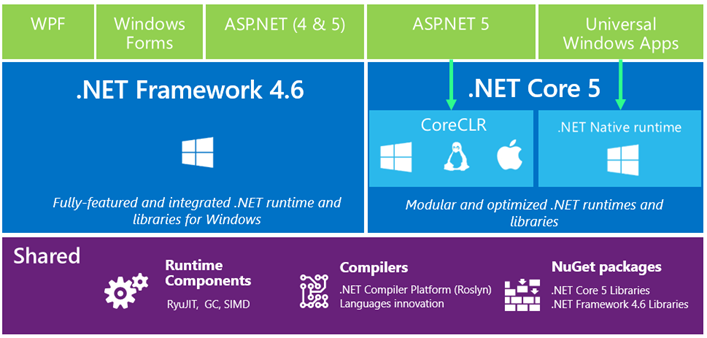
\includegraphics[width=15cm]{./images/UnderstandingNetCore}
  \captionsource{Übersicht .NET Framework \& .NET Core}{\url{https://blogs.msdn.microsoft.com/bethmassi/2015/02/25/understanding-net-2015/}}
\end{figure}


\subsubsection{5: Installation von .NET Core}
Aufgrund der Fehlermeldung haben wir nun versucht .NET Core auf dem Raspberry Pi zu installieren. Zur Zeit zu dem dieser Setup durchgeführt wurden, existierten keine offiziellen Microsoft-Quellen zur Installation von .NET Core unter Linux.

Um .NET Core unter Raspbian zu installieren, wird das bereits installierte Mono Framework benötigt. Anschliessend kann das \gls{acr:DNX} installiert werden. Diese Execution Environement beinhaltet alle notwendigen Libraries, um .NET Core Applikation auszuführen. Um  \gls{acr:DNX} zu installieren ist es am einfachsten den \gls{acr:DNVM} zu verwenden. Mit dem Version Manager können verschiedene Versionen des .NET Frameworks parallel installiert werden. \gls{acr:DNVM} bietet auch Möglichkeiten um zwischen den einzelnen Versionen einfach und schnell hin und her zu wechseln.

\textbf{Installation \gls{acr:DNVM}} \\
\begin{lstlisting}
curl -sSL https://raw.githubusercontent.com/aspnet/Home/dev/dnvminstall.sh | DNX_BRANCH=dev sh && source ~/.dnx/dnvm/dnvm.sh
\end{lstlisting}

\textbf{Installation  \gls{acr:DNX} .NET Core} \\
\begin{lstlisting}
sudo apt-get install libunwind8 gettext libssl-dev libcurl4-openssl-dev zlib1g libicu-dev uuid-dev
mozroots --import --sync
dnvm upgrade -u
dnvm install latest -r coreclr -u
\end{lstlisting}

Die beschriebenen Schritte konnten soweit problemlos durchgeführt werden. Anschliessend galt es das Test-Projekt auf das neue Build-System von  \gls{acr:DNX} umzustellen, welches mit .NET Core verwendet werden muss. Während dieser Umstellung hat sich gezeigt, dass der \gls{acr:DNVM} und die  \gls{acr:DNX} bereits wieder verworfen wurde und direkt durch die .NET Core CLI (Command Line Interface) abgedeckt werden\footnotemark[1]. Diese Umstellung wurde mit dem Wechsel der Version .NET Core RC1 auf .NET Core RC2 eingeführt. Zum Zeitpunkt dieser Arbeit bestand jedoch neben dem \gls{acr:DNVM} keine andere Möglichkeit .NET Core unter Linux / Mono zu installieren. Glücklicherweise konnte das .NET Core CLI zusammen mit der .NET Core Runtime dennoch via \gls{acr:DNVM} installiert werden.

\footnotetext[1]{\url{http://dotnet.github.io/docs/core-concepts/dnx-migration.html}}

Die nächste Herausforderung bestand anschliessend darin im neuen Build-System das korrekte Target-Framework zu definieren. Aufgrund dessen, dass es noch keinen ersten finalen Release von .NET Core CLI gibt, kursierten im Web verschiedenste Definitionen für das Target-Framework. Darunter zum Beispiel "`dotnet"' und "`dnxcore50"'.

Längere Recherchen und Analysen haben anschliessend zwei Fakten zu Tage gebracht, mit welchen wir nicht gerechnet hatten.
\begin{itemize}
\itemBfText{.NET Core in 32-Bit}{Aktuell gibt es von .NET Core keine 32-Bit Implementation. Sämtliche Raspberry Pi Modelle basieren auf einer ARM 32-Bit Architektur. Ausgenommen davon ist das neuste Model, der Raspberry Pi 3 Model B. Jedoch gibt es Raspbian aktuell nur in einer 32-Bit Version.}
\itemBfText{GrovePi NuGet Paket verwendet Windows-Only Funktionalitäten}{Das GrovePi NuGet Paket hat Abhängigkeiten zur Universal Windows Platform (UAP). Die Universal Windows Platform ist Teil der .NET Native Runtime und gibt es daher nur für Windows, nicht für Linux oder Mac OS. Die Abhängigkeit dieses NugGet Paketes von .NET Native besteht wahrscheinlich deshalb, weil die Library ursprünglich für die Verwendung mit Windows 10 Iot entworfen wurde.}
\end{itemize}


\subsubsection{6: Finaler Setup}
Aufgrund dieser letzten Erkenntnisse haben wir uns entschieden die Umsetzung auf Raspbian Jessie (32-Bit) mit dem regulären Mono-Framework zu realisieren. Aufgrund dessen, dass das GrovePi NuGet Paket nicht verwendet werden kann, muss der Zugriff, beziehungsweise die Kommunikation zwischen Raspberry Pi und GrovePi auf eine andere Art gelöst werden.


\subsection{Variante 2: Windows 10 IoT}
Windows 10 IoT ist eine Version des Betriebssystems von Microsoft, welches speziell für kleinere Geräte mit weniger Rechenleistung konzipiert wurde.

\subsubsection{Installation von Windows 10 IoT}
Microsoft bietet zwei Varianten an, um Windows 10 IoT auf einem Raspberry Pi zu installieren. Bei der ersten Variante wird das Betriebsystem direkt auf der SD-Karte installiert\footcite{install_win10iot_2016-04-25}. Dazu muss das Windows 10 IoT Core Dashboard auf einem Computer installiert werden. Anschliessend wird eine ISO Datei heruntergeladen, welches eine Installationsdatei beinhaltet welche über ein richtiges Windows 10 gestartet werden muss. Dies Datei kompiliert eine FFU Datei (Full Flash Update, Image-Datei) welche über das Core Dashboard installiert werden muss. Danach sollte der Raspberry Pi mit Windows 10 IoT gestartet werden können. \todo{Was bedeutet FFU?}

Leider startete das Raspberry Pi nach dem genannten Prozedere nicht, sondern blieb beim Rainbow Screen\footcite{RPi_Rainbowscreen_2016-04-25} hängen. Der Rainbow Screen ist Teil des Boot-Vorgangs und wird im Rahmen des \gls{acr:GPU}-Tests generiert.

\begin{figure}[H]
  \centering
  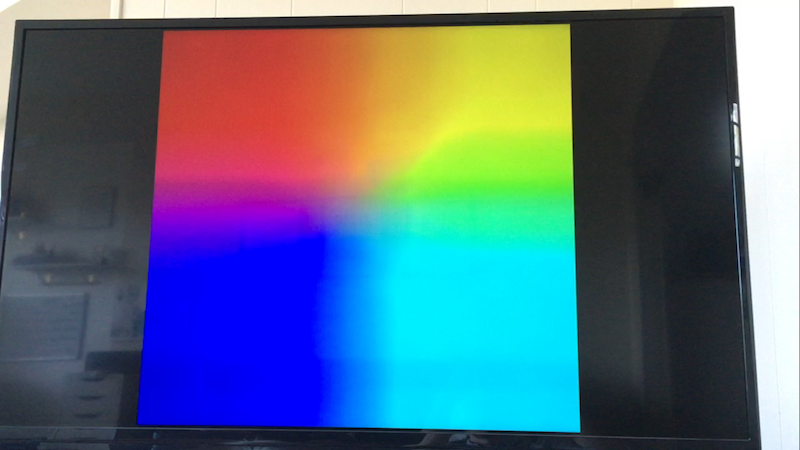
\includegraphics[width=0.8\textwidth]{./images/raspberry-rainbow-screen.png}
  \caption{Raspberry Pi rainbow screen}
\end{figure}

Die zweite Variante der Installation von Windows 10 IoT arbeitet mit dem NOOBS Installer (siehe \ref{sec:collect:fsharp:variant1:installation} \nameref{sec:collect:fsharp:variant1:installation}), welcher von der Raspberry Pi Foundation zur Verfügung gestellt wird. Zuerst muss NOOBS auf einer SD-Karte installiert (entpackt) und diese anschliessend in den Raspberry PI eingelegt werden. Vor dem Start muss der Raspberry Pi ans Internet angeschlossen werden, damit der Installer die notwendigen Dateien für die Installation herunterladen kann. Nach dem Anschluss des Raspberry Pi an die Stromversorgung startet der Installations-Manager in welchem Windows 10 Iot ausgewählt und installiert werden kann.

Die Installation über NOOBS war einiges einfach als diejenige über das Core Dashboard und war schlussendlich auch erfolgreich.

\subsubsection{Installation des Mono-Frameworks \& F\#}
Windows 10 IoT wird bereits mit dem .NET Micro Framework. Deshalb war keine Installation für .NET nötig.

\subsubsection{Installation von .NET Core}
Da für die Entwicklung für das GrovePi das .NET Core nötig ist, wurde nach einer Anleitung\footcite{How_to_run_DotNET_Core_Application_on_Pi2} versucht dieses zu installieren. Als erstes muss \gls{acr:DNVM} installiert werden, danach die CoreCLR\footcite{CoreCLR_2016-06-17}

\textbf{Installation \gls{acr:DNVM}} \\
\begin{lstlisting}
@powershell -NoProfile -ExecutionPolicy unrestricted -Command "`&{$Branch='dev';iex ((new-object net.webclient).DownloadString('https://raw.githubusercontent.com/aspnet/Home/dev/dnvminstall.ps1'))}"'
\end{lstlisting}

\textbf{Installation CoreCLR} \\
\begin{lstlisting}
c:\> dnvm install -r coreclr -arch x64 latest -u
\end{lstlisting}
\todo{@Simon: Meinsch da 64-Bit nimmi ah?}
Dies installiert die CoreCLR 32bit Version für einen ARM Prozessor, welcher auf dem Raspberry Pi verwendet wird. Leider funktionierte dies nicht. 

\begin{lstlisting}
Run Build Command:/usr/bin/make "cmTryCompileExec3109069071/fast"
/usr/bin/make -f CMakeFiles/cmTryCompileExec3109069071.dir/build.make CMakeFiles/cmTryCompileExec3109069071.dir/build
make[1]: Entering directory `/home/\dfrac{win10iot}{den}/coreclr/bin/obj/Linux.x64.Debug/CMakeFiles/CMakeTmp'
/usr/bin/cmake -E cmake_progress_report /home/win10iot/coreclr/bin/obj/Linux.x64.Debug/CMakeFiles/CMakeTmp/CMakeFiles 1
Building C object CMakeFiles/cmTryCompileExec3109069071.dir/testCCompiler.c.o
/usr/bin/clang-3.5   -Wall -std=c11    -o CMakeFiles/cmTryCompileExec3109069071.dir/testCCompiler.c.o   -c /home/win10iot/coreclr/bin/obj/Linux.x64.Debug/CMakeFiles/CMakeTmp/testCCompiler.c
Linking C executable cmTryCompileExec3109069071
/usr/bin/cmake -E cmake_link_script CMakeFiles/cmTryCompileExec3109069071.dir/link.txt --verbose=1
/usr/bin/clang-3.5   -Wall -std=c11     CMakeFiles/cmTryCompileExec3109069071.dir/testCCompiler.c.o  -o cmTryCompileExec3109069071 -rdynamic 
make[1]: Leaving directory `/home/win10iot/coreclr/bin/obj/Linux.x64.Debug/CMakeFiles/CMakeTmp'
\end{lstlisting}

\todo{Ist das oben die Fehlermeldung?}
Deshalb wurde entschieden, das Projekt mit der Variante 1: Rasbian Jessie fortzusetzen.

\section{Speicherung der Sensordaten}
Zum Abspeichern der Sensordaten haben sich verschiedene Datenformate angeboten. Um die Komplexität möglichst gering zu halten und maximale Flexibilität zu erreichen, haben wir uns entschieden die Sensordaten File-basiert abzuspeichern.

Neben \gls{acr:CSV} standen auch \gls{acr:JSON} oder \gls{acr:XML} zur Auswahl. Da die Daten in einem kontinuierlichen Stream geschrieben werden müssen haben wir uns schlussendlich für ein klassisches CSV-File entschieden. Dies bietet den Vorteil, dass neue Datensätze ohne Probleme laufend ans Ende der Datei angehängt werden können.

Bei \gls{acr:JSON} und \gls{acr:XML} ist dies nicht ohne weiteres möglich, da die Daten dort in Hierarchischer Form abgespeichert werden.


\section{Umsetzung}
In diesem Kapitel wird die konkrete Umsetzung der Problemstellung "`Sammeln von Sensordaten"' beschrieben.

\subsection{Verwendete Hardware}
Für die Realisierung wurden nachfolgend aufgelisteten Hardware-Komponenten verwendet.

\begin{figure}[H]
  \centering
  \includegraphics[width=10cm]{./images/_DSC2016}
  \caption{Der verwendete Raspberry Pi mit den Sensoren}
\end{figure}

\begin{itemize}
\item Raspberry Pi 2 Model B
\item Raspberry Pi 3 Model B
\item GrovePi Sensoren
\begin{itemize}
\item Temperature \& Humidity Sensor (GrovePi Port D3)
\item Sound Sensor (GrovePi Port A0)
\item Light Sensor (GrovePi Port A2)
\item Blue LED (GrovePi Port D4)
\end{itemize}
\end{itemize}




\subsection{Verwendete Software}
Für die Realisierung, beziehungsweise den Betrieb, wurden folgende Softwarekomponenten verwendet:

\begin{itemize}
\item Raspbian Jessie
\item GrovePi Firmware + Beispiele
\item Mono 4.2
\item NOOBS
\item F\# Interactive
\end{itemize}

\subsection{Dokumentation der Implementation}
Die konkrete Implementation der Problemstellung "`Sensordaten sammeln"' wird im Abschnitt \ref{sec:AnalyseCollection:ImplDoc} \nameref{sec:AnalyseCollection:ImplDoc} dokumentiert.

\subsection{Datentransfer zum Raspberry Pi}
Die kompilierten Sourcen wurden via Linux-Befehl "`scp"' auf den Raspberry Pi übertragen.

\begin{lstlisting}
scp -rp ./Raspberry.FGrove pi@raspberrypi.local:/home/pi/Development/FUP/
\end{lstlisting}

\subsection{Datentransfer vom Raspberry Pi}
Der Datentransfer vom Raspberry Pi auf einen anderen Computer wurde durch einen einfachen HTTP-Server auf Python-Basis bewerkstelligt. Python wurde bei der Installation des GrovePi automatisch mitinstalliert. Dadurch konnten wir den "`SimpleHTTPServer"' nutzen, welcher standardmässig mit Python ausgeliefert wird.

\begin{lstlisting}
python -m SimpleHTTPServer 8000
\end{lstlisting}


\subsection{Betrieb \& Starten der Applikation}
Damit der Raspberry Pi zum Sammeln von Sensordaten theoretisch auch unabhängig von einem Netzwerk betrieben werden könnte, wurde der Raspberry Pi als WiFi-Access-Point konfiguriert. Beim Start wird geprüft, ob ein bekanntes WiFi-Netzwerk verfügbar ist. Ist dies nicht der Fall, werden entsprechend die Konfigurationen für den WiFi-Access-Point geladen. Die Konfiguration dieses Access-Points, beziehungsweise Ad-Hoc-Netzwerkes, wurde anhand der Anleitungen von \hyperlink{http://lcdev.dk/2012/11/18/raspberry-pi-tutorial-connect-to-wifi-or-create-an-encrypted-dhcp-enabled-ad-hoc-network-as-fallback/}{Lasse Christiansen} und \hyperlink{http://slicepi.com/creating-an-ad-hoc-network-for-your-raspberry-pi/}{cpetty33} durchgeführt.


Mit diesem Setup kann nun jederzeit auf den Raspberry Pi zugegriffen und entweder die Anwendung gestartet / gestoppt oder die Daten heruntergeladen werden.

Für den Start der Anwendung musste ein zusätzliches Tool namens "`screen"' installiert werden. Mit diesem Tool ist es einfach möglich mehrere Hintergrundverarbeitungen zu starten, welche nicht automatisch beendet werden, sobald die aktuelle Session (SSH-Verbindung) terminiert wird.

\textbf{Start der Anwendung}
\begin{lstlisting}
ssh pi@raspberrypi.local (SSH into Raspberry Pi))
screen -S rpfs (create new screen session "`rpfs"')
python -m SimpleHTTPServer 8000 (start Python HTTP-Server)
Ctrl + a + c (create new window in current screen session)
sudo fsharpi --lib:/home/pi/Development/FUP/Raspberry.FGrove/libs "/home/pi/Development/FUP/Raspberry.FGrove/Program.fsx" (start F\# application)
ctrl + a + d (detach from current screen session)
\end{lstlisting}

\textbf{Beenden der Anwendung}
\begin{lstlisting}
ssh pi@raspberrypi.local (SSH into Raspberry Pi))
screen -r rpfs (attach to the existing screen session "`rpfs"')
ctrl + c (terminate F\# application)
exit (close current window in screen session)
ctrl + c (terminate Python HTTP-Server)
exit (closes current window and screen session)
\end{lstlisting}

\section{Dokumentation der Implementation}
\label{sec:AnalyseCollection:ImplDoc}
Nachfolgend werden die wichtigsten Punkte der einzelnen Komponenten dokumentiert.

\subsection{Komponenten}
Die Anwendung besteht aus den nachfolgend beschriebenen Teilkomponenten.

\begin{figure}[H]
  \centering
  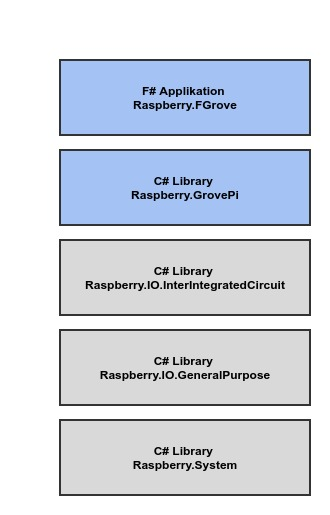
\includegraphics[width=6cm]{./images/Component-Overview}
  \caption{Komponentenübersicht}
\end{figure}

\begin{itemize}
\item Raspberry.FGrove (F\# Applikation)
\item Raspberry.GrovePi (C\# Library)
\item Raspberry.IO.InterIntegratedCircuit (C\# Library)
\item Raspberry.IO.GeneralPurpose (C\# Library)
\item Raspberry.System (C\# Library)
\end{itemize}


\subsection{Source Code}
Der Source Code wird in folgendem Git-Repository verwaltet: \hyperlink{https://github.com/Liechtathlet/FUP_Sem_IOT}{FUP\_Sem\_IOT}

\subsection{Raspberry.IO.InterIntegratedCircuit (C\# Library)}
Bei dieser Komponente handelt es sich um einen Klon / Fork der Teilkomponente "`Raspberry.IO.InterIntegratedCircuit"' des Git-Repositorys \hyperlink{https://github.com/raspberry-sharp/raspberry-sharp-io/tree/master/Raspberry.IO.InterIntegratedCircuit}{raspberry-sharp-io} von \hyperlink{https://github.com/raspberry-sharp}{Raspberry\#}.

Diese Library ist aktuell nicht als NuGet-Packet verfügbar und wurde spezifisch für .NET unter Mono optimiert. Die Library verwendet die NuGet-Packete "`Raspberry.IO.GeneralPurpose"' und "`Raspberry.System"', welche von Raspberry\# veröffentlicht und im genannten Git-Repository gepflegt werden.

Das Ziel dieser Library ist es, den Zugriff auf den \gls{acr:I2C}-Bus des Raspberry Pi zu abstrahieren / vereinfachen.

\subsection{Raspberry.GrovePi (C\# Library)}
Diese Komponente stellt unter Verwendung der Library "`Raspberry.IO.InterIntegratedCircuit"' spezifische Funktionalitäten für den Zugriff auf den GrovePi via \gls{acr:I2C} zur Verfügung.

Die Library besteht aus einer einzigen Wrapper-Klasse, welche die \gls{acr:I2C} und GrovePi spezifischen Elemente für die eingesetzten Sensoren abstrahiert. Über den \gls{acr:I2C}-Bus müssen spezifische Befehle gesendet werden, um die gewünschten Sensordaten auszulesen. Diese Befehle werden von einem Arduino auf dem GrovePi Board interpretiert und verarbeitet. Die zulässigen Befehlssequenzen wurden den Hersteller-Dokumentationen entnommen.

Die Daten, welche von den Sensoren zurückgegeben werden, sind meistens nicht direkt verwendbar, da diese noch in Rohform vorliegen. Der Temperatursensor gibt zum Beispiel keinen absoluten Wert in Grad Celsius oder Kelvin zurück. Die entsprechenden Rohwerte müssten über spezielle Formeln entsprechend den Hardwarekomponenten umgerechnet werden. Die Herstellerdokumentationen sind an dieser Stelle leider lückenhaft, wodurch die entsprechenden Umrechnungen nur teilweise durchgeführt werden konnten.

\begin{itemize}
\item \hyperlink{https://learn.adafruit.com/adafruits-raspberry-pi-lesson-4-gpio-setup/the-gpio-connector}{Raspberry Pi GPIO Connector}
\item \hyperlink{http://www.dexterindustries.com/GrovePi/engineering/port-description/}{GrovePi Port Description}
\item \hyperlink{http://www.dexterindustries.com/GrovePi/programming/grovepi-protocol-adding-custom-sensors/}{GrovePi Protocol and Adding Custom Sensors}
\item \hyperlink{https://github.com/DexterInd/GrovePi/blob/bfcaa57bb6ce2b5c4cb0057569ea38f3574f24cf/Firmware/Source/v1.2/grove_pi_v1_2_6/README.md}{GrovePi Firmware Documentation}
\item \hyperlink{http://www.seeedstudio.com/wiki/Grove_-_Sound_Sensor}{GrovePi Sound Sensor}
\item \hyperlink{http://www.seeedstudio.com/wiki/Grove_-_Temperature_and_Humidity_Sensor}{GrovePi Temperature \& Humidity Sensor}
\item \hyperlink{http://www.seeedstudio.com/wiki/Grove_-_Light_Sensor}{GrovePi Light Sensor}
\end{itemize}


Nachfolgend werden die verwendeten Befehlsfolgen aufgezeigt:

\textbf{I2C auf dem Raspberry}
\begin{lstlisting}
SDA-Pin: P1Pin03 (Nummer des SDA GPIO-Pins auf dem Raspberry Pi Board, notwendig für I2C, Data-Line)
SCL-Pin: P1Pin05 (Nummer des SCL GPIO-Pins auf dem Raspberry Pi Board, notwendig für I2C, Clock-Line)
I2C Device Address: 0x04
\end{lstlisting}

\textbf{Allgemeines Befehlsschema}
\begin{lstlisting}
Byte 0: 1 (Dummy, statischer Wert)
Byte 1: Command (ID der auszuführenden Aktion)
Byte 2: Pin (Nummer des anzusprechenden Pin auf dem GrovePi)
Byte 3: Data (Optional, Input-Daten)
Byte 4: Data (Optional, Input-Daten)
\end{lstlisting}

\textbf{Sound / Noise Sensor}
\begin{lstlisting}
Byte 0: 1 (Dummy)
Byte 1: 3 (Command: Analog-Read)
Byte 2: 0 (Pin: 0)
Byte 3: 0
Byte 4: 0
Result: 3 bytes (Sensordaten: Umgebungslautstärke)
\end{lstlisting}

\textbf{Temperature \& Humidity Sensor}
\begin{lstlisting}
Byte 0: 1 (Dummy)
Byte 1: 40 (Command: Read DHT-Sensor)
Byte 2: 3 (Pin: 3)
Byte 3: 0
Byte 4: 0
Result: 9 bytes (Sensordaten: Temperatur, Luftfeuchtigkeit)
\end{lstlisting}

\textbf{Light Sensor}
\begin{lstlisting}
Byte 0: 1 (Dummy)
Byte 1: 3 (Command: Analog-Read)
Byte 2: 2 (Pin: 2)
Byte 3: 0
Byte 4: 0
Result: 3 bytes (Sensordaten: Helligkeit / Lichtintensität)
\end{lstlisting}


\textbf{LED (On)}
\begin{lstlisting}
Byte 0: 1 (Dummy)
Byte 1: 2 (Command: Digital-Write)
Byte 2: 4 (Pin: 4)
Byte 3: 1 (Data: On)
Byte 4: 0
Result: -
\end{lstlisting}

\textbf{LED (Off)}
\begin{lstlisting}
Byte 0: 1 (Dummy)
Byte 1: 2 (Command: Digital-Write)
Byte 2: 4 (Pin: 4)
Byte 3: 0 (Data: Off)
Byte 4: 0
Result: -
\end{lstlisting}


Der GrovePi verarbeitet die eingehenden Befehle sequentiell. Damit sichergestellt ist, dass zum abgesetzten Befehl auch die korrekten Daten zurückgeliefert werden, wurde der Lock-Mechanismus von C\# verwendet. Dadurch wird der Zugriff auf den GrovePi so eingeschränkt, dass kein simultaner Zugriff mehr möglich ist.

\begin{lstlisting}
// Byte-Array for results
byte[] ret; 

// Create lock, if locked: wait till lock is released
lock (_locker) { 
	// Send command to GrovePi
	connection.Write (new[] { (byte)1, (byte)3, (byte)2, (byte)0, (byte)0 }); 
	
	// Wait a few ms (allows the arduino to collect the data)
	Thread.Sleep (10); 
	
	// Read the response
	ret = connection.Read (3); 
	
// release the lock
} 
\end{lstlisting}


\subsection{Raspberry.FGrove (F\# Applikation)}
\label{sec:AnalyseCollection:application}
Diese Komponente realisiert die Kern-Logik der Anwendung, die Sammlung und Speicherung der Sensordaten. Dazu wird die implementierte C\# Library "`Raspberry.GrovePi"' verwendet.

Pro Sensor wurde ein eigenständiger Timer implementiert, welche periodisch gestartet und anschliessend zurückgesetzt wird. Pro Timer wurde ein Event-Listener registriert, welcher die spezifischen Sensordaten ausliest und anschliessend in ein \gls{acr:CSV}-File schreibt.

Nachfolgend wird die Implementation exemplarisch für den "`Sound Sensor"' aufgezeigt:
\begin{lstlisting}
// Create timer for sound / noise sensor
let nTimer, nEventStream = startTimerAndCreateObservable 100 

// Subscribe to event
nEventStream |> Observable.subscribe (fun _ -> processNoiseEvent())
\end{lstlisting}

\textbf{startTimerAndCreateObservable}
\begin{lstlisting}
// Creates and starts a new timer and returns an observable event
let startTimerAndCreateObservable timerInterval =
    // Setup timer
    let timer = new System.Timers.Timer(float timerInterval)

    // Autoreset and enable
    timer.AutoReset <- true
    timer.Enabled <- true

    // Return observable event
    (timer,timer.Elapsed)
\end{lstlisting} 

\textbf{writeData}
\begin{lstlisting}
// Writes the sensordata to a file. If the file doesn't exists it will be created. Otherwise the data will be appended to the end of the file.
let writeData suffix (data:String) (date:DateTime) (location:String) = 
    let filepath = "./data/SensorData-" + suffix + ".csv"

    if not(File.Exists(filepath)) then
        printfn "Data-File doesn't exists, creating file"
        use streamWriter = new StreamWriter(filepath,false)
        streamWriter.WriteLine "Date;Time;SensorData;Location"
        streamWriter.Flush()
        streamWriter.Close()

    use streamWriter = new StreamWriter(filepath,true)
    [ date.ToString("dd.MM.yyyy");
      date.ToString("hh:mm:ss.fff");
      data;
      location]
    |> List.fold (fun r s -> r + s + ";") ""
    |> streamWriter.WriteLine

    streamWriter.Flush()
    streamWriter.Close()
\end{lstlisting} 

\textbf{readNoiseSensor}
\begin{lstlisting}
// Reads the data from the sound / noise sensor. 
let readNoiseSensor() = 
	grovePiWrapper.readNoiseSensorData()
\end{lstlisting}  
   
   
\textbf{processNoiseEvent}
\begin{lstlisting}
// Processes the timer event for the sound / noise sensor.
let processNoiseEvent() =
     let sensorValue = readNoiseSensor()
     writeData "N" (sensorValue.ToString()) DateTime.Now currentLocation
\end{lstlisting}

Die Daten werden in folgendem Format in die CSV-Dateien geschrieben:
\begin{lstlisting}
Date;Time;SensorData;Location
06.05.2016;11:55:30.344;68;Brun@Home;
06.05.2016;11:55:30.367;70;Brun@Home;
06.05.2016;11:55:30.403;69;Brun@Home;
06.05.2016;11:55:30.426;71;Brun@Home;
[...]
\end{lstlisting}